\subsection{Testing for Buffer overflow - OTG-INPVAL-014}
\subsubsection{BANK-APP}
\begin{longtable}[l]{ p{2.3cm} | p{.79\linewidth} }\hline
    & \textbf{BANK-APP}
    \\ \hline
    \textbf{Observation} & When a text file is uploaded with huge data without adhering to the format specified, the application crashes and keeps waiting for the response. \\
    \textbf{Discovery} &
        A large file was used to discover this vulnerability. Steps are as follows.
                \begin{itemize}
                    \item Open the application and go to the New Transaction page.
                    \item Set the Foxy Proxy standard to Burp Suite for all URLs under the tool tab in Firefox.
                    \item Open the Burp Suite and under proxy tab set the interception to on state.
                    \item Now upload a file with huge data.
                    \item Observe the Alerts tab as its get highlighted. It shows that the application crashed since the memory allocation failed. This creates a suspicion of buffer overflow. See Figure \ref{fig:burp_large_file_upload}.
                \end{itemize}
     \\
    \textbf{Likelihood} & Likelihood is high, since this uploading of file with huge data is quite easy to do and no technical knowledge is required. \\
    \textbf{Impact} & The impact is high since the application crashes without notifying the user about the reason behind it. \\
    \textbf{Recommen\-dations} & Files with huge data should not be parsed at all, by having a check on file size(both client side and server side).   \\ \hline
    \textbf{CVSS} &
        \begin{tabular}[t]{@{}l | l}
            Attack Vector           & \textcolor{red}{Network} \\
            Attack Complexity       & \textcolor{red}{Low}\\
            Privileges Required     & \textcolor{red}{None}\\
            User Interaction        & \textcolor{Green}{Required} \\
            Scope                   & \textcolor{red}{Changed} \\
            Confidentiality Impact  & \textcolor{Green}{None} \\
            Integrity Impact        & \textcolor{Green}{None} \\
            Availability Impact     & \textcolor{red}{High}
        \end{tabular}
    \\ \hline
\end{longtable}

\subsubsection{SecureBank}
\begin{longtable}[l]{ p{2.3cm} | p{.79\linewidth} }\hline
    & \textbf{SecureBank}
    \\ \hline
    \textbf{Observation} & When a text file is uploaded with huge data without adhering to the format specified, the application crashes and keeps waiting for the response. \\
    \textbf{Discovery} & Same as described for BANK-APP. \\
    \textbf{Likelihood} & Same as described for BANK-APP. \\
    \textbf{Impact} & Same as described for BANK-APP.  \\
    \textbf{Recommen\-dations} & Same as described for BANK-APP. \\ \hline
    \textbf{CVSS} & Same as described for BANK-APP.
    \\ \hline
\end{longtable}

\begin{figure}[ht]
	\centering
		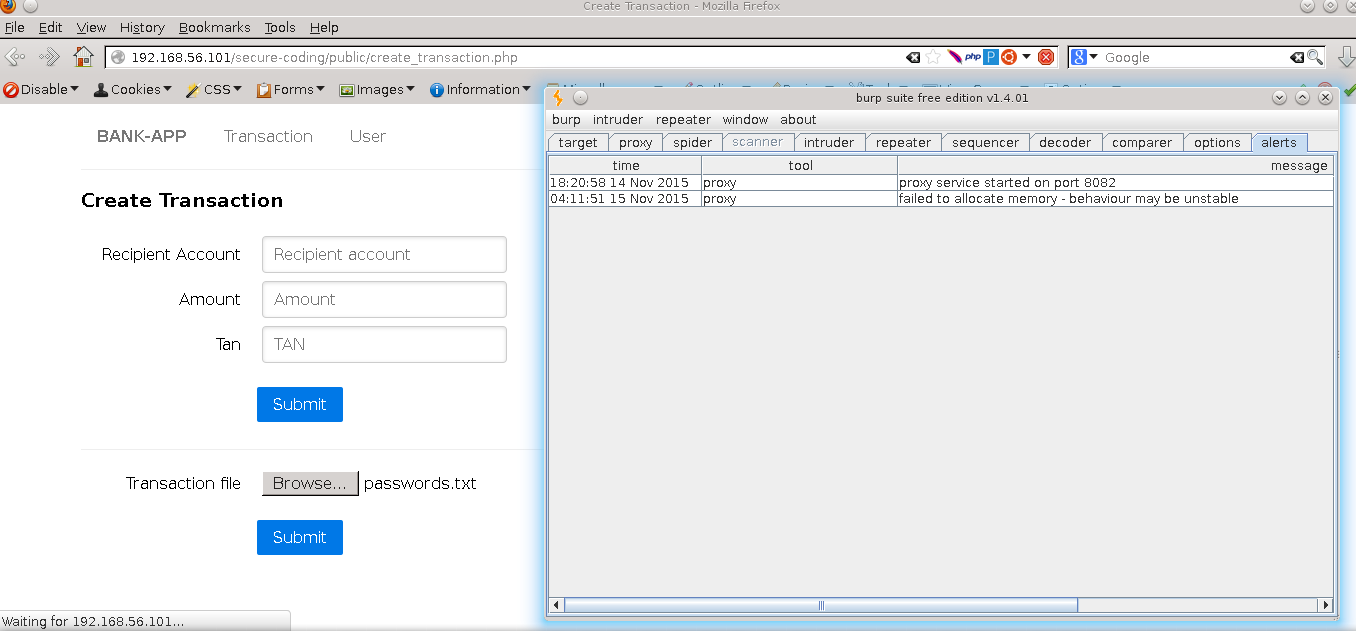
\includegraphics[width=.8\linewidth]{figures/OTG-INPVAL-014.png}
		\caption{BURP - Testing large file upload}
	\label{fig:burp_large_file_upload}
\end{figure}

\subsubsection{Comparison}
Neither applications perform well in handling big files leading to application crash, and thus suspectecting buffer overflow.
\clearpage